%\noindent {\bf Chapter editors:}~James Beacham, Giovanna Cottin, David Curtin, Jared Evans, Zhen Liu, Michael Ramsey-Musolf, Jessie Shelton, Brian Shuve \\
%\text{ \; }\\
%\noindent {\bf Contributors:}~Andreas Albert, Oliver Buchmueller, Alessandro Davoli, Andrea De Simone, Kristian Hahn, Jan Heisig, Thomas Jacques, Matthew McCullough, Stephen Mrenna, Marco Trovato, others
%\text{ \; }\\
%\text{ \; }\\

%%%%%%%%%%%%%%%%
%% JS: this new introduction is aimed at helping this document stand alone; I'd imagine in the final white paper a lot of these ideas would be introduced in the overall introduction.

\noindent LLPs arise in many well-motivated theories of physics beyond the SM, ranging from  well-established scenarios such as the minimal supersymmetric  SM (MSSM) to newer theoretical frameworks such as neutral naturalness and hidden sector dark matter.  Macroscopic decay lengths of new particles naturally arise from the presence and breaking of new symmetries, which can be motivated by cosmology (such as dark matter and baryogenesis) \cite{Bouquet:1986mq, Campbell:1990fa, Cui:2012jh, Barry:2013nva, Cui:2014twa, Ipek:2016bpf,Feng:2008ya,Baumgart:2009tn, Kaplan:2009ag,
  Chan:2011aa, Dienes:2011ja, Dienes:2012yz, Kim:2013ivd}, neutrino masses \cite{Helo:2013esa, Antusch:2016vyf,Graesser:2007yj, Graesser:2007pc, Izaguirre:2015pga,Maiezza:2015lza, Batell:2016zod,Cottin:2018kmq,Nemevsek:2018bbt}, as well as solutions to the hierarchy problem  \cite{Giudice:1998bp,Burdman:2006tz, Cai:2008au, Chacko:2005pe,Fan:2011yu,Barbier:2004ez, Csaki:2013jza,Arvanitaki:2012ps, ArkaniHamed:2012gw}; indeed, LLPs are generically a prediction of new weak-scale hidden sectors \cite{Chen:1995yu,Thomas:1998wy,Feng:1999fu,Strassler:2006im,Strassler:2006ri,Strassler:2006qa,Han:2007ae,Strassler:2008bv,Strassler:2008fv}.  A comprehensive search program for LLPs is therefore critical to fully leverage the LHC's immense capability to illuminate the physics of the weak scale and beyond. 
  
 The simplified models framework has proven to be a highly successful approach driving the development of  searches for new signatures at the LHC and allowing existing searches to be reinterpreted for many models beyond the one(s) initially targeted in the search. Comprehensive simplified models programs existing for scenarios featuring prompt decays of new particles \cite{ArkaniHamed:2005px,Knuteson:2006ha,ArkaniHamed:2007fw,Aaltonen:2007dg,Alwall:2008ag,Alwall:2008va,Alves:2011wf} or dark matter produced at colliders \cite{Petriello:2008pu,Dudas:2009uq,Goodman:2011jq,An:2012va,Frandsen:2012rk,Dreiner:2013vla,Cotta:2013jna,Abdallah:2015ter}.  Simplified models are so successful because the majority of search sensitivity is driven by only a few broad aspects of a given beyond-SM (BSM) signature such as the production process, overall production rate, and decay topology. Meanwhile, the sensitivity of searches is typically insensitive to other properties such as the spin of the particles involved~\cite{Edelhauser:2015ksa,Edelhauser:2014ena,Arina:2015uea,Kraml:2016eti}.


In order to extend the simplified models approach to LLP signatures in a systematic way, we develop a simplified models proposal which aims to ensure that experimental results are (i) {\em powerful}, covering as much territory as possible; (ii) {\em efficient}, reducing unnecessary redundancy among searches; (iii) {\em flexible}, so that they are broadly applicable to different types of models, and (iv) {\em durable}, providing a common framework for Monte Carlo simulation of signals, and facilitating the communication of results of LLP searches so that they may be compared and applied to new models for years to come. We elaborate on these goals in Section~\ref{sec:goals}.
We expect that this common framework will help illuminate gaps in coverage and highlight areas where new searches are needed, and we undertake such a study in Section~\ref{sec:experimentcoverage}. {\bf [BS:~I tried to make this less intro-y, but since the goals aren't fleshed out so fully in the introduction, I think there is still value in their enumeration here. I'm open to comments though!]}




In our work, we concentrate on establishing an initial basis of simplified models representative of theories giving rise to final states with one or two LLPs\footnote{Some models predict moderately higher LLP multiplicities, but the coverage of such signatures from 1-2 LLP searches is good provided the LLPs do not overlap in the detector. Our proposed simplified models are not, however, representative of high-multiplicity signatures such as dark showers (see Section~\ref{sec:simplified_future}).}.  The simplified model approach is very powerful for LLP signatures:~the typically lower backgrounds for displaced signatures allow searches to be highly inclusive with respect to other objects in the event or the identification of objects originating from the displaced vertex. This enables a single analysis to have sensitivity to a wide variety of possible models for LLP production and decay. Our efforts build on earlier work proposing simplified model programs for LLPs motivated by particular considerations such as SUSY or dark matter (DM) \cite{Heisig:2012zq,Liu:2015bma,Heisig:2015yla,Khoze:2017ixx,Mahbubani:2017gjh,Buchmueller:2017uqu}. 

We organize our simplified models in terms of {\bf LLP channels} characterized by a particular LLP production mode and a particular decay mode. Because the production and decay positions of LLPs are physically distinct\footnote{External detectors can also be used to search for ultra-long-lived neutral or milli-charged particles \cite{Haas:2014dda,Chou:2016lxi,Gligorov:2017nwh,Feng:2017uoz}. }, it is possible to factorize and consider separately their production and decay.\footnote{In addition to production and decay, a third consideration is the propagation of particles through the detector.  While particles that do not possess color charge undergo straightforward propagation, colored states, \emph{e.g.}, SUSY $R$-hadrons, or particles with exotic charges such as magnetic monopoles or quirks, typically engage in a more complicated and often very uncertain traverse through the detector.  The subtleties with colored LLPs will be discussed more in subsection \ref{sec:coloredLLPs}. A trickier question is how to best simulate such states:~since charged or colored LLPs interact with the detector material, there must be an interface between the detector simulation software and the program implementing decay. This will be discussed further in Sec.~\ref{sec:proposal}.} 
For each LLP channel, the lifetime of the LLP is taken to be a free parameter. We emphasize that the LLP channel defined here is \emph{not} the same as an experimental signature that manifests in the detector:~a single channel can give rise to many different signatures depending on where (or whether)\footnote{The case of detector-stable particles is understood to be included setting $c\tau\to\infty$. Apparently, in this case there is no dependence on the decay mode.
See section~\ref{sec:decmodes} for further details.} the LLP decays occur inside the detector, while a single experimental search for a particular signature could potentially cover many simplified model channels. In this document, we focus on the construction and simulation of a concrete basis of LLP simplified model channels; a partial mapping of existing searches into our basis of simplified models is discussed in Section~\ref{sec:experimentcoverage}, along with the highest-priority gaps in current coverage and proposals for new searches.

As discussed in the existing simplified models literature, simplified models have their own limited range of applicability \cite{Alves:2011wf,Abdallah:2015ter}. For example, the presentation of search results in terms of simplified models often assume 100\% branching fractions into particular final states. In a UV model where the LLP decays in a very large number of ways, none of the individual simplified model searches may be sufficient to constrain it. Similarly, if the LLP is produced in a UV model with other associated objects that spoil the signal efficiency (for example, the production of energetic, prompt objects collimated with the LLP such that the signal fails isolation or displacement criteria; this is particularly important for high-multiplicity or dark-shower scenarios), then the simplified model result does not apply. Nevertheless, the simplified models framework allows us to organize possible production modes and signatures in a systematic way and identify if there are any interesting signals or parts of parameter space that are missed by current searches. Search results presented in terms of simplified models also cover a wide range of UV models. Therefore, we present a proposal for simplified models here with the understanding that there exist scenarios where UV models remain important for developing searches and presenting results.

The basis of simplified models presented here is  a starting point, rather than a final statement:~the present goal is to provide a set of simplified models that covers many of the best-motivated and simplest models containing singly- and doubly-produced LLPs (and, by extension, many models with three to four relatively isolated LLPs as well). Simplified models by design do not include all of the specific details and subtle features that may be found in a given complete model.  Therefore, the provided list is meant to be expandable to cover new or more refined models as the LLP search program develops.  For instance,  extending the simplified model framework to separately treat final states with heavy-flavor particles is of high interest (in analogy with the prompt case \cite{Essig:2011qg,Brust:2011tb,Papucci:2011wy}); see Section~\ref{sec:simplified_future} for a discussion of this and other future opportunities.   High-multiplicity signatures such as dark showers or emerging jets present different experimental and theoretical issues. Also, a broader set of simplified models may be needed to present the results of experimental searches and to allow ready application of experimental results to UV models of interest. 


%%%%%%%%%%%%%%%%%%%%%%%%%%%%%%%
\section{Goals of the Present Simplified Model Framework}\label{sec:goals}
%%%%%%%%%%%%%%%%%%%%%%%%%%%%%%%

The purpose of the simplified model framework is to provide a simple, common language that experimentalists and theorists can use to describe theories of LLPs and the corresponding mapping between models and experimental signatures. We therefore want our simplified model space to:
%
\begin{enumerate}
%
\item  Use a minimal but sufficient set of models to cover a wide range of the best-motivated theories of LLPs;
\item  Furnish a simple map between models and signatures to enable a clear assessment of existing search coverage and possible gaps; 
\item Expand flexibly when needed to incorporate theories and signatures not yet proposed;
\item Provide a concrete Monte Carlo signal event-generation framework;
\item Facilitate the re-interpretation of searches by supplying a sufficiently varied set of standard benchmark models for which experimental efficiencies can be provided for validation purposes.
\end{enumerate}
%
Note that points \#1 and \#5 are somewhat in tension with one another:~we wish to have a compact set of models that can be the subject of systematic study in terms of experimental signatures, but expressing experimental results in terms of only this set of simplified models may make it challenging to re-interpret experimental searches for UV models that are not precisely described by one of the simplified models. In this section, we prioritize having a minimal set of simplified models for the purpose of studying experimental coverages and generating new search ideas, while we defer a discussion of simplified models in the presentation and
reinterpretation of search results to Chapter~\ref{sec:reint}.\footnote{We note that in general more benchmark models may be needed for enabling reliable re-interpretation than the minimal set discussed here. An example where an extended set of simplified models is used can be seen in the heavy stable charged particle (HSCP) re-interpretation in Section~\ref{sec:ch5-smsHSCP} (Table~\ref{tab:defModels}).}

In the following sections, we construct a proposal for a minimal basis of simplified models for events with one or two LLPs.
We begin with a discussion of the theories that dominate the predictions for LLPs, and identify a set of `umbrella' models that yield LLPs in Section~\ref{sec:motivated_theories}.  We next identify the relevant (simplified) production and decay modes for LLPs in Section~\ref{sec:building_blocks},  emphasizing that each production mode has a characteristic set of predictions for the number and nature of {\em prompt} objects accompanying the LLP.  In Section~\ref{sec:proposal} we combine these production and decay modes into our simplified model basis and highlight how different umbrella models naturally populate the various LLP channels.  Section~\ref{sec:library} and Appendix  \ref{sec:library_more}  presents a framework and instructions for how the best motivated simplified model channels can be simulated in Monte Carlo using a new model library outlined in Appendix \ref{sec:library_more}. 


%%%%%%%%%%%%%%%%%%%%%%%%%%%%%%%%%%%%%
\section{Existing Well-Motivated Theories for LLPs}\label{sec:motivated_theories}
%%%%%%%%%%%%%%%%%%%%%%%%%%%%%%%%%%%%%

Here we provide a brief distillation of many of the best-motivated theories with LLPs into five over-arching categories, focusing in particular on those that give rise to single and double production of LLPs at colliders.  We emphasize that each of these categories is a broad umbrella containing many different individual models containing LLPs; in many cases, the motivations and model details among theories within a particular category may be very different, but  tend to predict similar types of LLPs. In all cases, long lifetimes typically arise from some combination of hierarchies of scales in interactions that mediate decays; small couplings; and phase space considerations (such as small mass splittings between particles).

The UV umbrella models we consider are:
%
\begin{itemize}

\item {\bf Supersymmetry-like theories (SUSY).}~This category contains models
  with multiple new particles carrying SM gauge charges and a variety
  of allowed cascade decays. LLPs can arise as a result of approximate
  symmetries (such as $R$-parity \cite{Barbier:2004ez} or indeed SUSY itself in the case
  of gauge mediation \cite{Dimopoulos:1996vz}) or through a hierarchy of mass scales (such as
  highly off-shell intermediaries in split SUSY \cite{ArkaniHamed:2004fb}, or
  nearly-degenerate multiplets \cite{Chen:1995yu,Thomas:1998wy,Byrne:2003sa}, as in anomaly-mediated SUSY breaking \cite{Feng:1999fu}).  Our terminology
  classifies any non-SUSY models with new SM gauge-charged particles, such
  as composite Higgs or extra-dimensional models, under the SUSY-like
  umbrella because of the prediction of new particles above the weak scale with SM charges.  In this category, LLP production is typically dominated by
  SM gauge interactions, whether of the LLP itself or of a heavy
  parent particle that decays to LLPs.

\item {\bf Higgs-portal theories (Higgs).}~In this category, LLPs couple predominantly to the SM-like Higgs boson.  This possibility is well-motivated because the SM Higgs field provides one of the leading renormalizable portals for new gauge-singlet particles to couple to the SM, and the experimental characterization of the Higgs boson leaves much scope for couplings of the Higgs to BSM physics \cite{Khachatryan:2014jba,Aad:2015pla}.  The most striking signatures here are exotic Higgs decays  to low-mass particles  \cite{Curtin:2013fra} (as in many Hidden Valley scenarios \cite{Strassler:2006im,Strassler:2006ri}), which can arise in models of neutral naturalness \cite{Chacko:2005pe,Burdman:2006tz,Craig:2015pha} and DM \cite{Silveira:1985rk}.  
The Higgs is also special in that it comes with a rich set of associated production modes in addition to the dominant gluon-fusion process, with vector-boson fusion (VBF) and Higgs-strahlung (VH) production modes allowing novel opportunities for triggering on and suppressing backgrounds to Higgs-portal LLP signatures. Indeed, in many scenarios where LLPs are produced in exotic Higgs decays, associated production modes can be the only way of triggering the event.

\item {\bf Gauge-portal theories (ZP).}~This category contains scenarios where new vector mediators can produce LLPs. These are similar to Higgs models, but where the vector mediator is predominantly produced from $q\bar{q}$-initiated final states without other associated objects. Examples include models where both SM fermions and LLPs carry a charge associated with a new $Z'$ (for a review, see Ref.~\cite{Langacker:2008yv}), as well as either Abelian or non-Abelian ``dark'' photon or dark $Z$ models \cite{Holdom:1985ag} in which the couplings of new vector bosons to the SM are mediated by kinetic mixing. Scenarios with LLPs coupled to new gauge bosons are well motivated by theories of DM, particularly models with significant self-interactions \cite{Feng:2009hw,Buckley:2009in,Tulin:2012wi} and/or sub-weak mass scales \cite{Boehm:2003hm,Boehm:2003ha,Pospelov:2007mp,ArkaniHamed:2008qp,ArkaniHamed:2008qn}.

\item {\bf Dark-matter theories (DM):}~Non-SUSY and hidden-sector DM scenarios are collected in this category, which encompasses models where the cosmological DM is produced as a final state in the collider process. Examples of multi-component DM theories include models of new electroweak multiplets \cite{Thomas:1998wy,Cirelli:2005uq,Cirelli:2009uv,FileviezPerez:2008bj}, strongly interacting massive particles (SIMPs) \cite{Hochberg:2015vrg}, inelastic dark matter \cite{TuckerSmith:2001hy}, and models with DM coannihilation partners \cite{Griest:1990kh,Baker:2015qna,Khoze:2017ixx}. In many of these models, the collider phenomenology and LLP lifetime can be tied to the DM relic abundance. The main feature distinguishing this category from the Higgs and gauge scenarios above is that dark matter, \emph{i.e.,} missing energy ($\slashed{E}_{\rm T}$), is a necessary and irreducible component of such signatures  \cite{Strassler:2006im,Strassler:2006ri,Baumgart:2009tn,Falkowski:2010cm,Bai:2011jg,Primulando:2015lfa,Bai:2015nfa,Izaguirre:2015zva,Khoze:2017ixx,Buchmueller:2017uqu,Garny:2017rxs,Davoli:2017swj}. 

\item {\bf Heavy neutrino theories (RH$\nu$):}~The see-saw mechanism of SM neutrino mass generation predicts new right-handed neutrino (RHN) states \cite{Minkowski:1977sc,Yanagida:1979as,Mohapatra:1979ia,Glashow:1979nm,Mohapatra:1986bd}. If the RHNs have masses in the GeV to TeV range, they typically have a long lifetime and can be probed at the LHC \cite{Keung:1983uu,Ferrari:2000sp,Basso:2008iv,Atre:2009rg,Perez:2009mu,Nemevsek:2011hz,Helo:2013esa,Izaguirre:2015pga,Maiezza:2015lza,Batell:2016zod,Nemevsek:2016enw,Accomando:2016rpc,Accomando:2016sge,Caputo:2017pit,Accomando:2017qcs,Cottin:2018kmq,Nemevsek:2018bbt,Helo:2018qej}. Examples of well-motivated, UV-complete models with RHNs include the neutrino minimal SM ($\nu$MSM) \cite{Asaka:2005an,Asaka:2005pn} and the left$-$right symmetric model \cite{Pati:1974yy,Mohapatra:1974gc,Senjanovic:1975rk,Senjanovic:1978ev}.  Characteristic features of models in this category are LLPs produced singly via SM neutral and charged current interactions, and lepton-rich signatures in terms of prompt and displaced objects (often in association with quarks); in extended models like left$-$right symmetric models, production through new right-handed $W$ and $Z$ bosons can lead to production of between one and four LLPs, and cascade decays between RHNs can lead to phenomena such as doubly displaced decays. RHNs can also be produced via Higgs decays \cite{Graesser:2007yj, Graesser:2007pc,Maiezza:2015lza,Accomando:2016rpc,Das:2017rsu,Caputo:2017pit}.

\end{itemize}
%
Note that it is possible for a given model to fit into two of the umbrella UV model categories. For example, a SUSY theory with stable lightest SUSY particle (LSP) could have the LSP serve as a dark matter candidate, while alternatively DM could be a new electroweak multiplet, giving rise to SUSY-like signatures \cite{Thomas:1998wy,Cirelli:2005uq,Cirelli:2009uv,FileviezPerez:2008bj}. Thus, these should not be considered as exclusive categories, but rather as umbrella scenarios that motivate particular classes of signatures (such as new SM gauge-charged particles in the SUSY-like category, or presence of $\slashed{E}_{\rm T}$ in DM models).


%
In developing our simplified model framework below, we will construct maps between these UV model categories and the simplified model channels to illuminate some of the best-motivated combinations of production and decay modes for LLPs. This  allows us in upcoming work to focus on the most interesting channels and assess their coverage in the work of the Experimental Coverage Working Group reported in Section~\ref{sec:experimentcoverage}.



%%%%%%%%%%%%%%%%%%%%%%%%%%%%%%%%%%%%%%%%%%%%%%
\section{The Simplified Model Building Blocks}\label{sec:building_blocks}
%%%%%%%%%%%%%%%%%%%%%%%%%%%%%%%%%%%%%%%%%%%%%%


As discussed above, production and decay can largely be factorized in LLP searches. This allows us to specify the relevant production and decay modes for LLP models separately; we then put them together and map the space of models into the umbrella categories of motivated theories.

%%%%%%%%%%%%%%%%%%%%%%%%%%%%%%%%%%%
\subsection{Production Modes}
\label{SM:secProduction_modes}
%%%%%%%%%%%%%%%%%%%%%%%%%%%%%%%%%%%

Motivated by our over-arching UV frameworks, we can identify a minimal set of interesting production modes for LLPs.
These production modes determine LLP signal yield both by relating the  LLP production cross section to meaningful theory parameters such as gauge charges or Higgs couplings, and by determining the kinematic distribution of the LLP.  Additionally, a given production mechanism will also  make clear predictions for the number and type of {\em prompt} objects accompanying the LLP(s).  These prompt accompanying objects (AOs) can be important for both triggering on events with LLPs and for background rejection, particularly when the LLP has a low mass or decays purely hadronically.  Schematic diagrams for each production mode are shown in Fig.~\ref{fig:feyndiagram}.

%
\begin{itemize}

\item {\bf Direct Pair Production (DPP):}~Here the LLP is dominantly pair-produced non-resonantly from SM initial states.  This is most straightforwardly obtained when the LLP is charged under a SM gauge interaction.  
%, it can be directly produced via the corresponding gauge boson. 
In this case, an irreducible production cross section is then specified by the LLP gauge charge and mass.  DPP can also occur in the presence of a (heavy) $t$-channel mediator (e.g., an initial quark$-$antiquark pair may exchange a virtual squark to pair produce bino-like neutralinos); in this case the production cross section is a free parameter.

\item {\bf Heavy parent (HP):}~ In this case the LLP can be produced in the decay of a heavy parent particle that is itself pair produced from the $pp$ initial state. The production cross section is essentially a free parameter, and is indirectly specified by the gauge charges and masses of the heavy parent particles. Heavy parent production gives very different kinematics for the LLP than direct pair production, and will often produce additional prompt accompanying objects in the rapid cascade decays of the parents.

\item {\bf Higgs (HIG):}~The LLP is produced through its couplings to the SM-like Higgs boson.  This case has an interesting interplay of possible production modes. The dominant production  is via  gluon fusion, which features no associated objects beyond initial state radiation (ISR); owing to its role in electroweak symmetry breaking, however, the Higgs has associated production modes (VBF, VH), each with its own characteristic features. The best prospects are for LLP masses below $m_h/2$, in which case the LLPs can be produced on-shell in SM-like Higgs-boson decays. LLPs with heavier masses can still be produced via an off-shell SM-like Higgs, albeit at lower rates. The LLP can be pair produced or singly produced through the Higgs portal depending on the model; an LLP $X$ can also be produced in association with $\slashed{E}_{\rm T}$ via $h\rightarrow XX+\slashed{E}_{\rm T}$ or $h\rightarrow X+\slashed{E}_{\rm T}$. The cross section (or, alternatively, the Higgs branching fraction into the LLP) is a free parameter of the model. The Higgs mass can also be taken as a free parameter:~there exist many theories that predict new exotic scalar states (such as the singlet scalar extension to the SM \cite{Silveira:1985rk}), and these new states can be produced through the same production modes as the SM Higgs.


\item {\bf Heavy resonance (RES):}~Here the LLP is produced in the decay of an on-shell resonance, such as a heavy $Z'$ gauge boson initiated by $q\bar{q}$ initial state. Note that production via an off-shell resonance is kinematically similar to the direct production (DPP) above.  As with HIG, the LLP can be pair-produced or singly-produced (potentially in association with missing energy). In RES models, ISR is the dominant source of accompanying prompt objects. Models with new heavy scalars could conceivably fall into either RES or HIG; the main determining factor according to our organizational scheme is whether the scalar possesses Higgs-like production modes such as VBF and VH. Note that heavy resonance decays to SM particles also occur in these models and, searches for such resonances \cite{Khachatryan:2016zqb,Sirunyan:2016iap,Aaboud:2017yvp,Sirunyan:2017dnz,Aaboud:2017buh,Aaboud:2018juj,Aaboud:2018zba} may complement the sensitivity for decays to LLPs.

\item {\bf Charged current (CC):}~In models with weak-scale right-handed neutrinos, the LLP can be produced in the leptonic decays of $W/W'$. Single production is favored.  Prompt charged leptons from the charged-current interaction are typical prompt objects accompanying the LLP.
\end{itemize}
%
%%%%%%%%%%%%%%%%%%%%%%%%
\begin{figure}[t]
\centerline{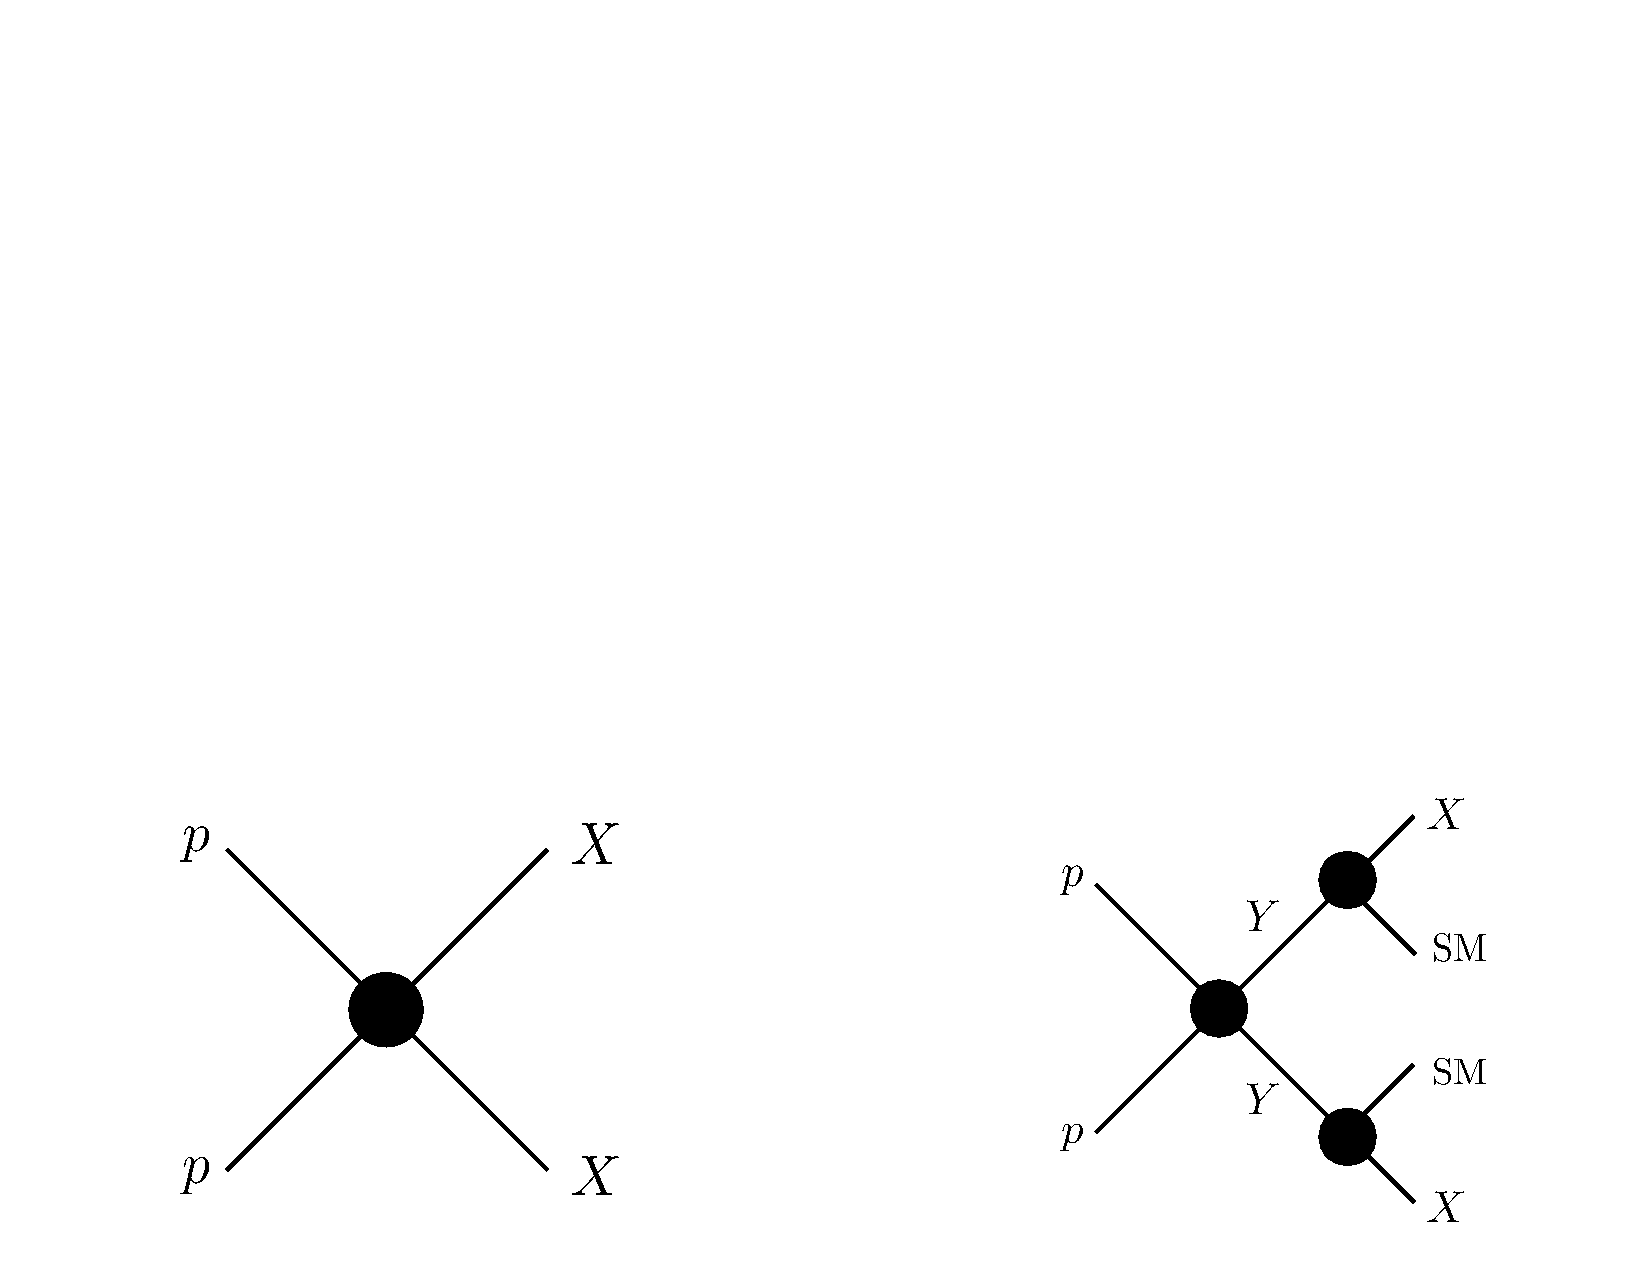
\includegraphics[width=\textwidth]{figures/feyndiagram_row1.pdf}}
\vspace{0.8cm}
\centerline{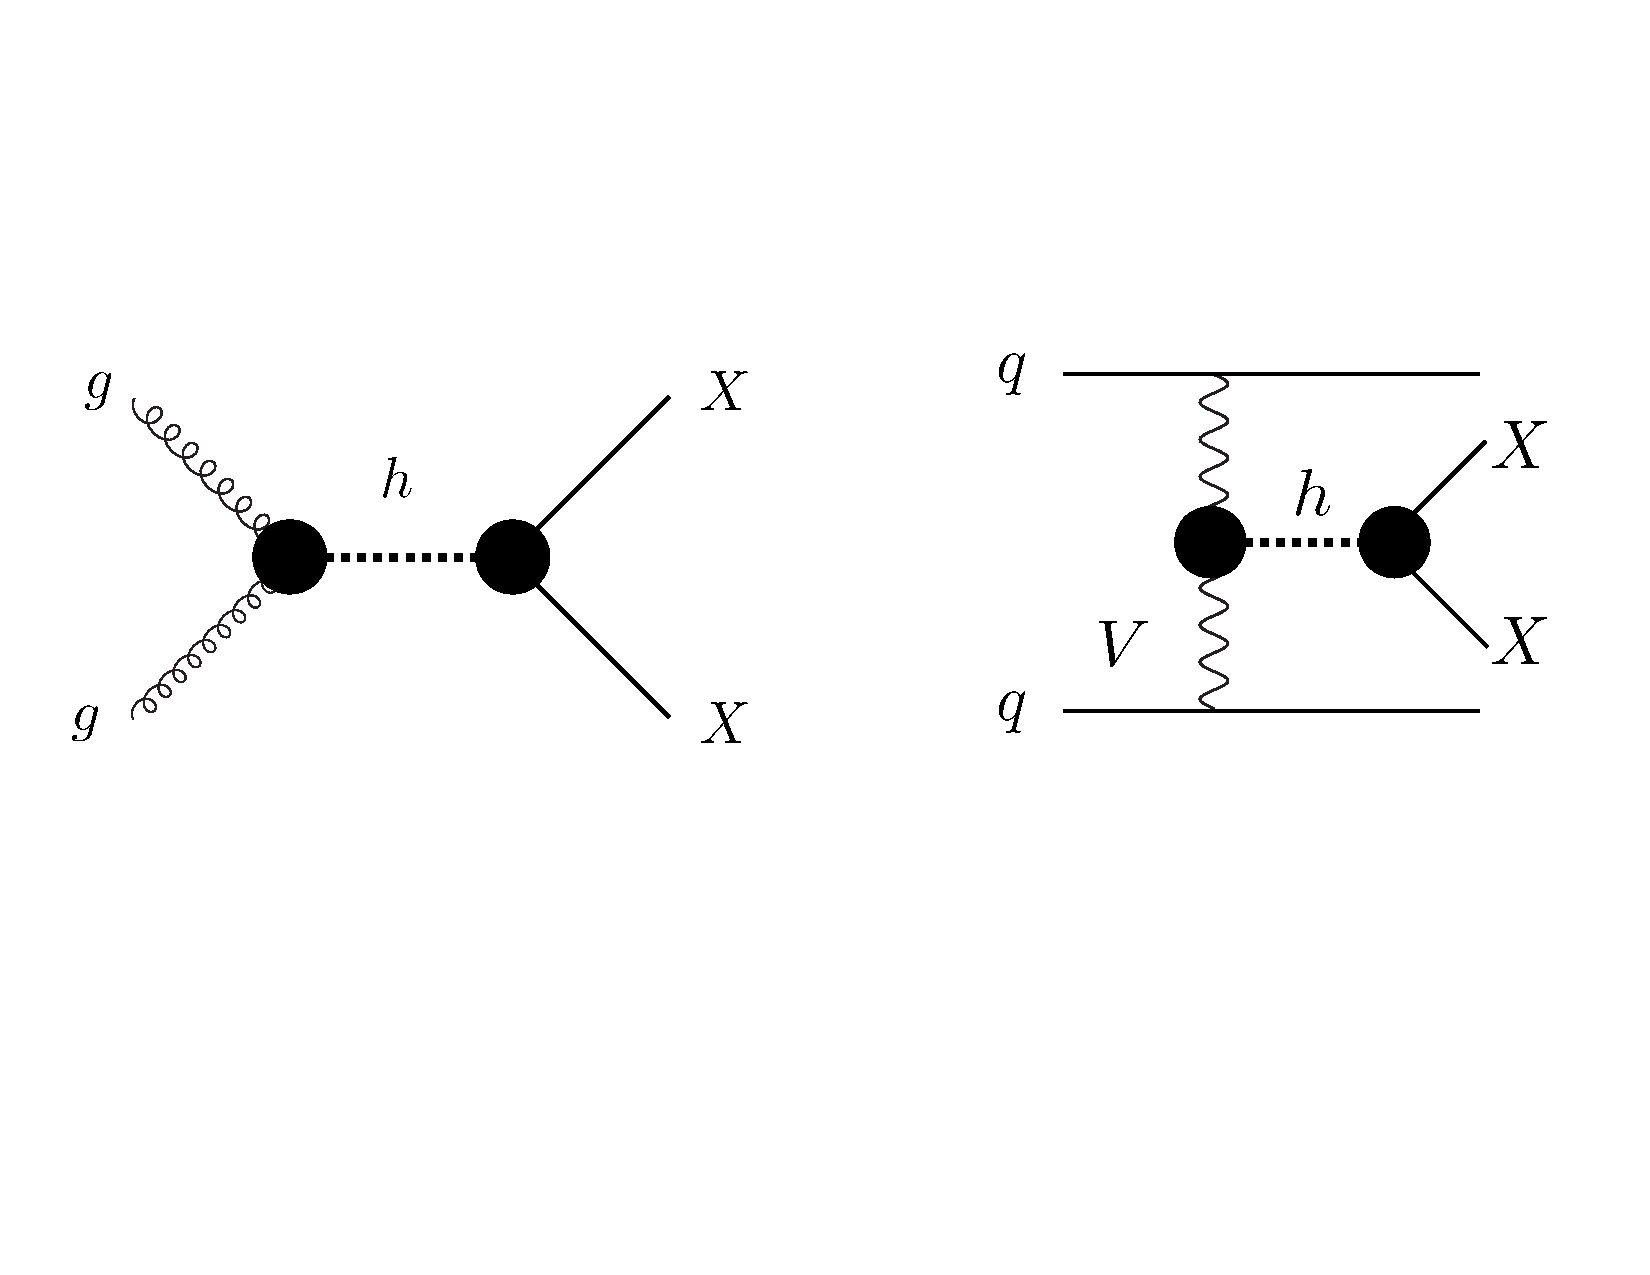
\includegraphics[width=\textwidth]{figures/feyndiagram_row2.pdf}}
\vspace{0.8cm}
\centerline{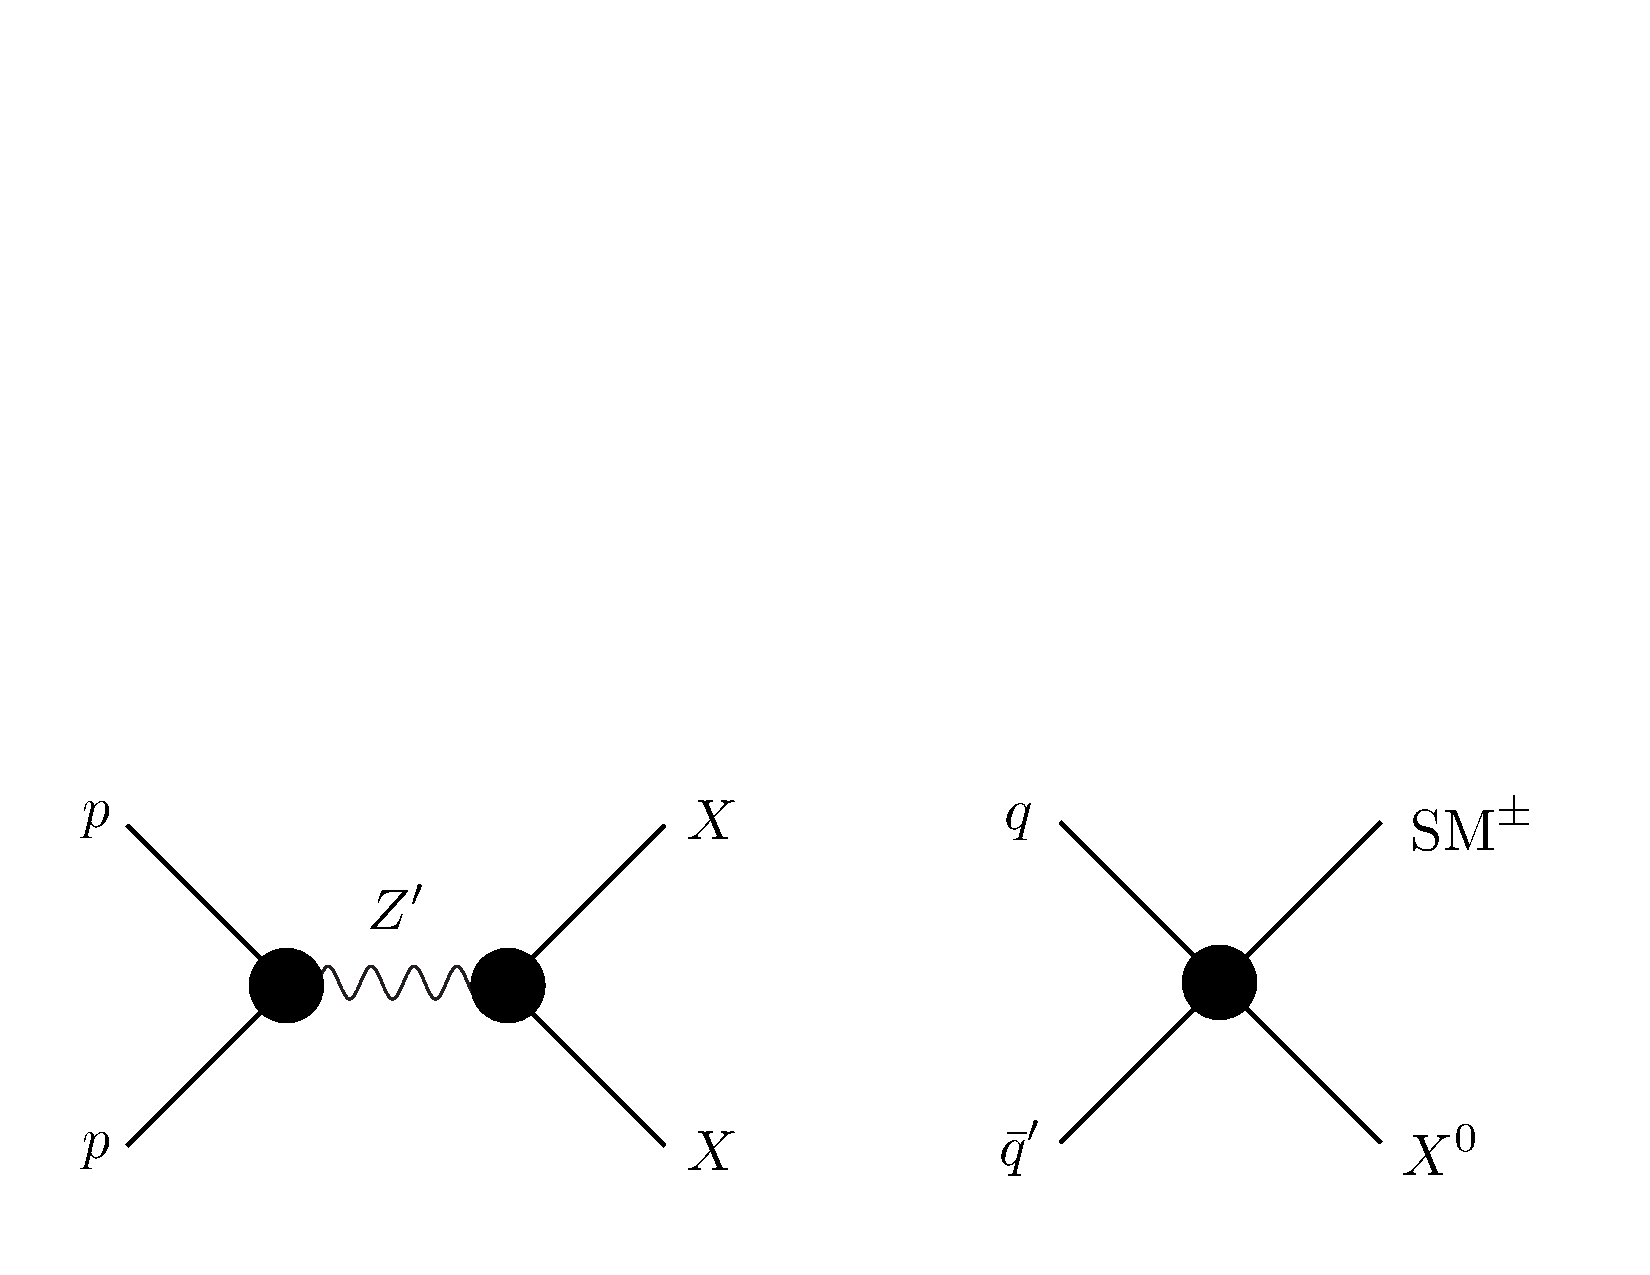
\includegraphics[width=\textwidth]{figures/feyndiagram_row3.pdf}}
  \caption{Schematic illustrations of LLP production modes in our simplified model framework. From top to bottom and left to right:~direct pair production (DPP); heavy parent (HP); Higgs modes (HIG), including gluon fusion and VBF production (not shown here is $VH$ production); heavy resonance (RES); charged current (CC).}
  \label{fig:feyndiagram}
\end{figure}
%%%%%%%%%%%%%%%%%%%%%%%%%

It is important to note that each of the above production mechanisms has its own ``natural'' set of triggers to record the signal. For example, HIG production can be accompanied by forward jets or leptons that are characteristic of VBF or VH production. Similarly,  CC production  often result in prompt charged leptons,  while HP production comes with associated hard objects from the heavy-parent decay. However, the reader should be cautioned that this does not necessarily mean that the ``natural'' trigger is the \emph{optimal} one for a particular signal:~for example, the HIG modes suggest the use of VBF- or VH-based triggers, but if the LLP decays leptonically, it might be more efficient to trigger on the lepton from the LLP decay. Thus, the final word on which trigger is most effective for a given simplified model depends on the production mode as well as the nature and kinematics of the LLP decay. The prompt associated objects of each production mode could still, however, be used to extend sensitivity to the model.

We also comment that some models may span several production modes. For example, a charged LLP that is part of an electroweak multiplet and nearly degenerate with a stable, neutral component \cite{Chen:1995yu,Thomas:1998wy,Feng:1999fu,
Cirelli:2005uq,Ibe:2006de,Cirelli:2009uv,FileviezPerez:2008bj,Buckley:2009kv,Mahbubani:2017gjh} gives both DPP signatures (via $pp\rightarrow \chi^+\chi^-$) and CC production (via associated production $pp\rightarrow\chi^\pm\chi^0$). Comprehensive coverage of each of the above production modes will allow for a conservative determination of sensitivity for models that span many production modes.


%%%%%%%%%%%%%%%%%%%%%%%%%%
\subsection{Decay Modes}\label{sec:decmodes}
%%%%%%%%%%%%%%%%%%%%%%%%%%


We now characterize a list of LLP decay modes. As we attempt to construct
a minimal, manageable set of decay-mode building blocks, it is important to keep in mind that a given experimental search for LLPs can frequently be
sensitive to a variety of possible LLP decay modes. As a result, it is not always necessary to divide LLP signatures into as many exclusive processes as might otherwise be needed for prompt signatures.

The fact that LLP searches can be sensitive to many LLP decay modes is, in part,
because LLPs that decay far from the collision point offer fewer
avenues for particle identification, (\emph{e.g.,} for an LLP decaying
inside of the calorimeter, most decay products are reconstructed as missing
energy, or an energy deposition in the calorimeter); consequently, particle identification
criteria are typically relaxed in comparison to requirements on searches without
displaced objects. Indeed, these ``loose'' collider objects can
differ significantly from the corresponding ``tight'', prompt objects. This leads to more 
inclusive analyses that can cover a wider range of signatures with a single search.


 Additionally,  backgrounds for LLP searches
are often small. As a result,  tight identification and/or reconstruction
criteria typically found in exclusive prompt analyses are  no longer needed to suppress
backgrounds. For example, ATLAS has a displaced vertex search
sensitive to di-lepton and multi-track vertices that are relatively
inclusive with respect to other objects originating from near the displaced vertex
\cite{Aad:2015rba}. Similarly, CMS has an analysis sensitive to
events with one each of a high-impact-parameter muon and electron without reconstructing a vertex or any other objects
\cite{CMS-PAS-EXO-16-022}. For these examples, the backgrounds are sufficiently low that other requirements may be relaxed and the specific decay mode of the LLP may not be too important so long as certain objects (such as muons) are present or the decay occurs in a specific location. An even more extreme example in this regard is the search for highly-ionizing tracks sensitive to electrically and color-charged LLPs. While the searches are primarily targeted to detector-stable particles (heavy stable charged particles or $R$-hadrons) they can also be used to probe intermediate lifetimes for which only a certain fraction of LLPs traverse the tracker before decaying (see \emph{e.g.}~\cite{Garny:2017rxs}). Both because of low backgrounds as well as modified particle identification criteria compared to prompt searches, LLP searches can often be inclusive and therefore covered by a more limited range of simplified models.

In some cases, however, the topology of a decay does matter. One potentially important factor
 that influences the sensitivity of a search to a particular model is whether
 the LLP decays into two SM objects vs.~three, because the kinematics of multi-body
decay are distinct from two-body decay and this may affect the 
acceptance of particular search strategies.  An additional simplified model 
  featuring a three-body decay of the LLP may consequently be needed to span
  the space of signatures.
  
Below, we describe an irreducible set of decay modes that can be used to
characterize LLP signatures for various LLP charges (including neutral, electrically charged, and colored). For each, we also provide an explicit example for how the decay would appear in a particular UV model. {\bf We  emphasize that the following decay modes are defined
  loosely with the understanding that their signatures will also be representative of similar related decay modes; for example
  $2j$ can also be a proxy for $3j$ because searches for
  multi-body hadronic LLP decays can be sensitive to both.} It
should also be noted that we are not recommending searches to be
optimized to the exact, exclusive decay mode because that could
suppress sensitivity to related but slightly more complicated decay chains.


\begin{itemize}
\item {\bf Di-photon decays:}~The LLP can decay resonantly to
  $\gamma\gamma$ (like in Higgs-portal models or left$-$right symmetric models
  \cite{Dev:2016vle}) or to
  $\gamma\gamma+\mathrm{invisible}$ (in dark matter models). This
  latter mode stands as a proxy for other $\gamma\gamma+X$ decays
  where the third object is not explicitly reconstructed. \emph{Example:~a 
  singlino decaying to a singlet (which decays to $\gamma\gamma$) and 
  a gravitino in Stealth SUSY \cite{Fan:2011yu}.}

\item {\bf Single photon decays:}~The LLP decays to
  $\gamma+\mathrm{invisible}$ (like in SUSY models).  The SUSY signal mandates a
  near-massless invisible particle, while other models allow for
  a heavy invisible particle, as can arise in theories of dark matter
  \cite{Weiner:2012cb,Primulando:2015lfa}. \emph{Example:~a bino decaying to photon plus gravitino in gauge-mediated
  models of SUSY breaking~\cite{Dimopoulos:1996yq}.}
%dark matter framework can come with a heavy final state particle.

\item {\bf Hadronic decays:}~The LLP can decay into two jets ($jj$)
  (like in Higgs and gauge-portal models, or RPV SUSY), $jj$ +
  invisible (SUSY, dark matter, or neutrino models), or $j$ +
  invisible (SUSY). Here, ``jet'' ($j$) means either a light-quark parton,
  gluon, or $b$-quark. This also encompasses decays directly into
  hadrons (for example, LLP decay into $\pi^+$ plus an invisible 
  particle  \cite{Chen:1995yu,Thomas:1998wy,Feng:1999fu}).
   \emph{Example:~a scalar LLP decaying to $b\bar{b}$
  due to mixing with the SM Higgs boson, as in models of
  neutral naturalness}. 

\item {\bf Semileptonic decays:}~The LLP can decay into a lepton + 1 jet (such as in leptoquark models)
  or 2 jets (like in SUSY or neutrino models). \emph{Example:~a right-handed neutrino decaying to a left-handed
   lepton and an on- or off-shell hadronically decaying $W$ boson (or $W'$ boson in a left$-$right
   symmetric model) \cite{Keung:1983uu}. }

\item {\bf Leptonic decays:}~The LLP can decay into
  $\ell^+\ell^-(+\mathrm{invisible})$, or
  $\ell^\pm+\mathrm{invisible}$ (as in Higgs-portal, gauge-portal,
  SUSY, or neutrino models). $\ell$ may be any flavor of charged
  lepton, but the decays are lepton flavor-universal and (for
  $\ell^+\ell^-$ decays) flavor-conserving. \emph{Example:~a wino decaying
  to a neutralino and an on- or off-shell leptonic Z boson in SUSY \cite{Barbier:2004ez}.}

\item {\bf Flavored leptonic decays:}~The LLP can decay into
  $\ell_\alpha+\mathrm{invisible}$, $\ell_\alpha^+\ell_\beta^-$ or
  $\ell_\alpha^+\ell_\beta^-+\mathrm{invisible}$ where flavors
  $\alpha\neq\beta$ (as in SUSY or neutrino models). \emph{Example:~a neutralino decaying to two
   leptons and a neutrino in $R$-parity-violating SUSY \cite{Barbier:2004ez}; or a right-handed neutrino decaying to 
   two leptons and a neutrino \cite{delAguila:2008cj}.}
\end{itemize}

In all cases, both the LLP mass and proper lifetime are free
parameters.  Therefore, the case of detector-stable particle is automatically included by taking
any of the above decay modes and setting $c\tau\rightarrow\infty$.\footnote{As mentioned 
earlier in this limit the decay mode becomes 
irrelevant. However, an exception is the search for particle that are stopped 
inside the detector material and decay out-of-time.}
We emphasize that, depending on the location of the LLP within the
detector, these decay modes may or may not be individually
distinguishable:~a displaced di-jet decay will look very different from
a displaced di-photon decay in the tracker, but nearly identical if the
decay occurs in the calorimeter.  We are identifying here promising
channels, as distinct from detector signatures. 

As an example of how the above listed decay modes cover the most important
experimental signatures, we consider a scenario of an LLP decaying to
top quarks. This scenario is very well-motivated (for instance, with
long-lived stops in SUSY) and might appear to merit its own decay
category of an LLP decaying to one or more top quarks. 
However, the top quark immediately decays to final states
that \emph{are} covered in the above list, giving a semileptonic
decay ($t\rightarrow b\ell^+\nu$) and a hadronic decay ($t\rightarrow
bjj$), and so the above model-independent LLP decay modes cover this
important scenario. Similarly, LLP decays to four or more final states are typically 
covered by the above inclusive definitions of decay modes; this provides 
motivation not to over-optimize
experimental searches to the specific, exclusive features of a
particular decay mode.

While it would be ideal to have separate experimental searches for
each of the above decay modes (when distinguishable), it is rare for
specific models to allow the LLP to decay in only one manner; instead,
as in the above example of an LLP decaying to a top quark,
 a number of decay modes are
typically allowed with corresponding predictions for the branching
fractions. As another example, if a LLP couples to the SM via mixing with the
SM Higgs boson, then the LLP decays via mass-proportional couplings
giving rise to $b$- and $\tau$-rich signatures. If, instead, the LLP
decays through a kinetic mixing as in the case of dark photons or $Z$
bosons, then the LLP can decay to any particle charged under the weak
interactions, giving rise to a relatively large leptonic branching
fraction in addition to hadronic decay modes. This allows some level
of prioritization of decay modes based on motivated UV-complete
models; for example, the Higgs-portal model prioritizes searches for heavy-flavor
quarks and leptons in LLP decay. Ultimately, however, it is desirable to retain independent
sensitivity to each individual decay mode as much as possible.  Indeed, for each decay
mode listed above, models exist  for which the given
decay mode would be the discovery channel. 
\linebreak


\noindent {\bf Invisible Final-State Particles:}~Where invisible
particles appear as products of LLP decays, additional
model dependence arises from the unknown nature and mass of the
invisible particle. The invisible particle could be a SM neutrino, DM,
an LSP in SUSY, or another beyond-SM particle. The phenomenology depends
strongly on the mass splitting, $\Delta \equiv M_{\rm LLP}-M_{\rm
  invisible}$. If $\Delta \ll M_{\rm LLP}$ (\emph{i.e.,} $M_{\rm
  LLP}\sim M_{\rm invisible}$), the spectrum is squeezed and the decay
products of the LLP are soft. This could, for instance, lead to
signatures such as disappearing tracks or necessitate the use of ISR
jets to trigger on the LLP signature. If the mass splitting is large,
$M_{\rm invisible}\ll M_{\rm LLP}$, then the signatures lose their
dependence on the invisible particle mass.

We suggest three possible benchmarks:~a squeezed spectrum with $\Delta
\ll M_{\rm LLP}$ (example:~a nearly degenerate chargino-neutralino pair,
giving rise to soft leptons or disappearing tracks \cite{Chen:1995yu,Thomas:1998wy,Feng:1999fu,
Cirelli:2005uq,Ibe:2006de,Cirelli:2009uv,FileviezPerez:2008bj,Buckley:2009kv,Mahbubani:2017gjh});
 a massless invisible state, $\Delta = M_{\rm LLP}$
(example:~a next-to-lightest SUSY particle (NLSP) decaying to SM
particles and a massless gravitino in gauge-mediated
SUSY breaking \cite{Dimopoulos:1996vz,Ambrosanio:1997rv,Delgado:2007rz,Meade:2010ji,
Allanach:2015cia,Evans:2016zau,Allanach:2016pam});
 and an intermediate splitting corresponding to a democratic
mass hierarchy, $\Delta \approx M_{\rm LLP}/2$ (example:~NLSPs in mini-split
SUSY \cite{Arvanitaki:2012ps,ArkaniHamed:2012gw,Liu:2015bma}).

%%%%%%%%%%%%%%%%%%%%%%%%%%%%%%%%%%%%
\section{A Simplified Model Proposal}\label{sec:proposal}
%%%%%%%%%%%%%%%%%%%%%%%%%%%%%%%%%%%%

In this section, we present a compact set of simplified model channels that, broadly speaking, covers the space of theoretical models in order to motivate new experimental searches. Such a minimal, compact set may not be optimal for reinterpretation of results (where variations on our listed production and decay modes may influence signal efficiencies and cross-section sensitivities), but rather provides a convenient characterization of possible signals to ensure that no major discovery mode is missed. These models may therefore serve as a starting point for systematically understanding experimental coverage of LLP signatures and devising new searches, but may need to be extended in future for the purposes of facilitating reinterpretation. We undertake an in-depth discussion of these topics in  Section~\ref{sec:reint}.

We classify LLPs according to their SM gauge charges, as these dictate
the dominant or allowed LLP production modes and can give rise
to different signatures (for example, disappearing tracks and
hadronized LLPs). We separately consider LLPs that 
are:~(a)~neutral, (b)~electrically
charged but color neutral, and (c)~color charged. In the latter case,
it is important to distinguish between the long-lived parton (which carries a QCD charge)
that hadronizes prior to decay,
and the physical LLP, which is a color-singlet $R$-hadron. The decays of the $R$-hadron are 
still dominated by the parton-level processes.

All of the following models have the LLP mass and lifetime as free parameters. For heavy-parent production, the parent mass is an additional parameter, while for invisible decays, several different benchmarks for mass splittings between LLP and invisible final state may have to be separately considered as described in Section~\ref{sec:decmodes}. The cross section may have  a theoretically well-motivated target value depending on  UV-model parameters, but phenomenologically can generally be taken as a free parameter.

We emphasize that in spite of the many simplified model
channels proposed below, a small number of experimental LLP searches can
have excellent coverage over a wide range of channels (for certain lifetime ranges). Ultimately, the goal in future work will be
to  identify whether there are other searches that could
have a similarly high impact on the space of simplified models, and  identify where the gaps in coverage are.

%%%%%%
\subsection{Neutral LLPs}
%%%%%%

The simplified model channels for neutral LLPs are shown in Table
\ref{tab:neutral_LLP}, where $X$ indicates the
LLP.

 
 In our proposal, which we expect to be the first iteration of the simplified
model framework, it is sufficient to consider as ``jets'' each of the
following:~$j=u,d,s,c,b,g$. It is worth commenting that $b$-quarks pose
unique challenges and opportunities. Since $b$-quarks are themselves
LLPs, they appear with an additional displacement relative to the LLP
decay location. They also often give rise to soft muons in their
decays, which could in principle lead to additional trigger or
selection possibilities.  However, these subtleties can be addressed
in further refinements of the simplified models; we discuss this further in Section
\ref{sec:simplified_future}. Similarly, we consider $e$,
$\mu$, and $\tau$ to be included in the header of ``leptons'', with the proviso that
searches should be designed where possible with sensitivity to each.
 
When multiple production modes are specified in one row of the table, this means that multiple
 especially well-motivated production channels give rise to similar
signatures. Typically only one of these production modes will actually need to
be included when developing a search, but we sometimes include multiple different production modes
as individuals may variously prefer one over the other. 


In each entry of the table, we indicate which umbrella category of well-motivated models
(Section~\ref{sec:motivated_theories}) can predict a particular
$(\mathrm{production})\times(\mathrm{decay})$ mode.  An asterisk (*) on
the umbrella model indicates that $\slashed{E}_{\rm T}$ is required in the decay. A dagger (${}^\dagger$) indicates that this particle production $\times$ decay scenario is not present in the \emph{simplest and most minimal} implementations of the umbrella model, but could be present in extensions of the minimal models. While
the Higgs signatures are best motivated for the SM-like 125 GeV Higgs, exotic Higgses
of other masses can still have the same production modes and so $m_H$ can be taken
as a free parameter.
%
\begin{table}
\begin{center}
\begin{tabular}{ |c|c|c|c|c|c|c| } 
 \hline
\backslashbox{Production}{Decay} & $\gamma\gamma(+\mathrm{inv.})$ & $\gamma+\mathrm{inv.}$ & $jj(+\mathrm{inv.})$ & $jj\ell$ & $\ell^+\ell^-(+\mathrm{inv.})$ & $\ell_\alpha^+\ell_{\beta\neq\alpha}^-(+\mathrm{inv.})$\\
\hline\hline
DPP:~sneutrino pair & ${}^\dagger$ & SUSY & SUSY & SUSY & SUSY & SUSY\\
 \hline
 HP:~squark pair, $\tilde{q}\rightarrow jX$ & $ {}^\dagger$  & SUSY & SUSY & SUSY & SUSY & SUSY\\
 or gluino pair $\tilde g\rightarrow jjX$ &&&&&&\\
 \hline
HP:~slepton pair, $\tilde{\ell}\rightarrow\ell X$ & ${}^\dagger$ & SUSY & SUSY & SUSY & SUSY & SUSY\\
 or chargino pair, $\tilde{\chi}\rightarrow WX$ &&&&&&\\
 \hline 
% HIG:~$h(h')\rightarrow XX$ & Higgs (DM)  &  & Higgs (DM) &  & Higgs (DM) & \\
 HIG:~$h\rightarrow XX$ & Higgs, DM*  & ${}^\dagger$ & Higgs, DM* & RH$\nu$ & Higgs, DM* &RH$\nu$* \\
  or $\rightarrow XX+\mathrm{inv.}$ &&&&& RH$\nu$* &\\
 \hline 
 %HIG:~$h(h')\rightarrow X+\mathrm{inv.}$ & DM  &  & DM &  & DM & \\
 HIG:~$h\rightarrow X+\mathrm{inv.}$ & DM*, RH$\nu$  & ${}^\dagger$ & DM* & RH$\nu$ & DM* &${}^\dagger$ \\
  \hline
   RES:~$Z(Z')\rightarrow XX$ & $Z'$, DM*  & ${}^\dagger$ & $Z'$, DM* & RH$\nu$ & $Z'$, DM* &$ {}^\dagger$\\
  or $\rightarrow XX+\mathrm{inv.}$ &&&&&&\\
 \hline 
 RES:~$Z(Z')\rightarrow X+\mathrm{inv.}$ & DM  & ${}^\dagger$ & DM &  RH$\nu$ & DM & ${}^\dagger$\\
  \hline
   CC:~$W(W')\rightarrow \ell X$ & ${}^\dagger$  & ${}^\dagger$ & RH$\nu$* & RH$\nu$ & RH$\nu$* & RH$\nu$* \\
  \hline
\end{tabular}
%
\end{center}
\caption{{\bf Simplified model channels for neutral LLPs.} The LLP is indicated by $X$. Each row shows a separate production mode and each column shows a separate possible decay mode, and therefore every cell in the table corresponds to a different simplified model channel of (production)$\times$(decay). We have cross-referenced the UV models from Section~\ref{sec:motivated_theories} with cells in the table to show how the most common signatures of complete models populate the simplified model space. The asterisk (*) shows that the model definitively predicts missing energy in the LLP decay. A dagger (${}^\dagger$) indicates that this particle production $\times$ decay scenario is not present in the \emph{simplest and most minimal} implementations of the umbrella model, but could be present in extensions of the minimal models. When two production modes are provided (with an ``or''), either simplified model can be used to cover the same experimental signatures.  }\label{tab:neutral_LLP}
\end{table}

We remind the reader that the production modes listed in Table
\ref{tab:neutral_LLP} encompass also the associated production of
characteristic prompt objects. For example, the Higgs production modes
not only proceed through gluon fusion, but also through vector boson
fusion and $VH$ production, each of which results in associated prompt
objects such as forward jets in VBF, and leptons or missing
energy in $VH$. All of the production modes listed in Table
\ref{tab:neutral_LLP} could be accompanied by ISR jets that aid in
triggering or identifying signal events. It is therefore important
that searches are designed to exploit such associated prompt objects
whenever they can improve signal sensitivity, especially with regard to triggering.

To demonstrate how to map full models onto the list of simplified
models (and vice-versa), we consider a few concrete cases. For
instance, if we consider a model of neutral naturalness where $X$ is a
long-lived scalar that decays via Higgs mixing (for instance, $X$
could be the lightest quasi-stable glueball), then the process where
the SM Higgs $h$ decays  $h\rightarrow XX$, $X\rightarrow b\bar{b}$
would be covered with the Higgs production mechanism and a di-jet
decay. Entirely unrelated models, such as the case where $X$ is a bino-like
neutralino with RPV decays  $h\rightarrow XX$, $X\rightarrow j jj $ could be covered
with the same simplified model because most hadronic LLP searches
do not have exclusive requirements on jet multiplicity. Similarly, a hidden-sector model with
a dark photon, $A'$, produced in $h\rightarrow A'A'$,
$A'\rightarrow f\bar{f}$ would also give rise to the di-jet signature
when $f$ is a quark, whereas it would populate the $\ell^+\ell^-$
column if $f$ is a lepton. Finally, a scenario with multiple hidden-sector states 
$X_1$ and $X_2$, in which $X_2$ is an LLP and $X_1$ is a
stable, invisible particle, could give rise to signatures like
$h\rightarrow X_2 X_2$, $X_2\rightarrow X_1jj$ that would be covered by the
same Higgs production, hadronic decay simplified model; however, we
see how $\slashed{E}_{\rm T}$ can easily appear in the final state,
and that the LLP decay products may not all be hadronic. Therefore, the simplified models in Table
\ref{tab:neutral_LLP} can cover an incredibly broad range of
signatures, but only if searches are not overly optimized to
particular features such as $\slashed{E}_{\rm T}$ and
resonant LLP reconstruction\footnote{This should not, of course, be interpreted as saying that searches
  shouldn't be done that exploit these features. Instead, our position is that
  experiments should bear in mind the range of topologies and models
  covered by each cell in Table \ref{tab:neutral_LLP} when designing
  searches, and that some more inclusive signal regions should be established where possible.}.
  

\subsection{Electrically Charged LLPs:~$|Q|=1$}\label{sec:EMcharge}

For an electrically charged LLP, we need to consider far fewer production modes because of the irreducible gauge production associated with the electric charge. We still consider a heavy-parent scenario where the heavy parent has a QCD charge, as this could potentially dominate the production cross section, see \emph{e.g.}~\cite{Heisig:2012zq}. We summarize our proposals in Table \ref{tab:charged_LLP}.

 Note that we lump all resonant production into the $Z'$ simplified model.  The reason is that the SM Higgs cannot decay into two on-shell charged particles due to the model-independent limits from LEP on charged particles masses, $M\gtrsim75-90$ GeV (see, for example, Ref.~\cite{Abbiendi:2003yd}).   Similarly, there are fewer decay modes because of the requirement of charge conservation. 

For concreteness, we recommend using $|Q|=1$ as a benchmark for charged LLPs for the purpose of determining allowed decay modes. 
Although other values of $Q$ are possible, these often result in cosmologically stable charged relics or necessitate different decay modes than those listed here.   LLPs with $|Q|=1$ are also motivated within SUSY \cite{Chen:1995yu,Thomas:1998wy,Feng:1999fu} and 
within Type-III seesaw models of neutrino masses \cite{Bajc:2006ia,Bajc:2007zf,Franceschini:2008pz,Arhrib:2009mz}.
We note that there exist already dedicated searches for heavy quasi-stable charged particles with non-standard charges \cite{Aad:2015kta,Khachatryan:2016sfv}; because those searches are by construction not intended to be sensitive to the decays of the LLP, the existing models are sufficient for characterizing these signatures and they do not need to be additionally included in our framework.

For massive particles with $|Q|=1$ with intermediate or large lifetimes such that the LLP traverses a significant part (or all) of the tracker the highly-ionizing track of the LLP provides a prominent signature. This can be exploited for an efficient background suppression while keeping identification and/or reconstruction criteria as loose and, hence, inclusive as possible. In particular, for decay-lengths of the order of or larger than the detector size the signature of highly-ionizing tracks and anomalous time-of-flight (\emph{i.e.}~searches for heavy stable charged particles) constitute an important search strategy covering a large range of lifetimes present in the parameter space of theoretically motivated models. While the searches for heavy stable charged particles are largely inclusive with respect to additional objects in the event they depend strongly on the velocity of the LLP\@. For $\beta\to1$ one looses the discriminating power against minimally ionizing particles, while for too small velocities, $\beta\lesssim0.5$, the reconstruction becomes increasingly difficult due to timing-issues. It is therefore important to include the heavy parent production scenario which covers a much larger kinematic range than direct production alone resulting in a much wider range of signal efficiencies~\cite{Heisig:2015yla}.


\begin{table}
\begin{center}
\begin{tabular}{ |c|c|c|c|c|} 
 \hline
\backslashbox{Production}{Decay} & $\ell+\mathrm{inv.}$ &  $jj(+\mathrm{inv.})$ & $jj\ell$ & $\ell\gamma$ \\
\hline\hline
DPP:~chargino pair & SUSY & SUSY & SUSY & ${}^\dagger$ \\
or slepton pair & DM* & DM* & &\\
\hline
HP:~$\tilde{q}\rightarrow j X$ & SUSY & SUSY & SUSY &${}^\dagger$ \\
& DM* & DM* & &\\
\hline
RES:~$Z'\rightarrow XX$ & Z', DM*& Z', DM* & Z'  &${}^\dagger$ \\
\hline
CC:~$W'\rightarrow X+\mathrm{inv.}$ & DM* & DM* & RH$\nu$ &${}^\dagger$\\
\hline
\end{tabular}
\end{center}
\caption{{\bf Simplified model channels for electrically charged LLPs, $|Q|=1$.} The LLP is indicated by $X$. Each row shows a separate production mode and each column shows a separate possible decay mode, and therefore every cell in the table corresponds to a different simplified model channel of (production)$\times$(decay). We have cross-referenced the ``well-motivated'' UV models from Section~\ref{sec:motivated_theories} with cells in the table to show how the most common signatures complete models can be linked to the simplified model space. The asterisk (*) shows that the model definitively predicts missing energy in the LLP decay. A dagger (${}^\dagger$) indicates that this particle production $\times$ decay scenario is not present in the \emph{simplest and most minimal} implementations of the umbrella model, but could be present in extensions of the minimal models. When two production modes are provided (with an ``or''), both production simplified models can be used to cover the same experimental signatures.  }\label{tab:charged_LLP}
\end{table}

While the signatures in Table \ref{tab:charged_LLP} form a minimal set, they also encompass some scenarios that merit special comment. One of these is the disappearing track signature \cite{Chen:1995yu,Thomas:1998wy,Feng:1999fu,Cirelli:2005uq,Ibe:2006de,Cirelli:2009uv,FileviezPerez:2008bj,Buckley:2009kv,Mahbubani:2017gjh}, in which a charged LLP decays to a nearly degenerate neutral particle. The lifetime is long in this scenario due to the tiny mass splitting between the two states. Formally, these are included in the chargino or slepton pair-production modes in Table \ref{tab:charged_LLP} with decays to $\ell+\mathrm{inv.}$ or $q\bar{q}'+\mathrm{inv.}$ taken in the limit where the splitting between the charged LLP and the invisible final state is of $\mathcal{O}(200\,\,\mathrm{MeV})$. In the case of a hadronic decay, $X$ decays to a soft pion that is very challenging to reconstruct and so the track simply disappears. This is an important scenario that is already the topic of existing searches \cite{CMS:2014gxa,Aaboud:2017mpt}. As the degeneracy between the charged LLP and the neutral  state is relaxed, other signatures are possible; this parameter range is well motivated both by SUSY and DM models with coannihilation \cite{Griest:1990kh,Baker:2015qna,Khoze:2017ixx}.

Finally, we comment on the challenges of simulating the charged LLP simplified models. Because the LLP interacts with the detector material before the decay, the simulation of the LLP propagation is important in correctly modelling the experimental signature. The subsequent decay of the LLP must either be hard-coded into the detector simulation, or allow for an interface with programs such as Pythia 8 to implement the decays. We discuss the challenges of simulating signals for LLPs with electric or color charge in Section \ref{sec:geant}.

\subsection{LLPs with Color Charge}
\label{sec:coloredLLPs}

LLPs with charges under the strong interactions are more constrained than even electrically charged LLPs. Because of the non-Abelian nature of the strong interactions, the gauge pair-production cross section of the LLP is specified by the LLP mass and its representation under the color group, $\mathrm{SU}(3)_{\rm C}$. 
We do not include production via a heavy parent particle here because that cross section is unlikely to dominate the total production rate at the LHC\@.

\begin{table}
\begin{center}
\begin{tabular}{ |c|c|c|c|c|}
 \hline
\backslashbox{Production}{Decay} & $j+\mathrm{inv.}$ &  $jj(+\mathrm{inv.})$ & $j\ell$ & $j\gamma$ \\
\hline\hline
DPP:~squark pair & SUSY & SUSY & SUSY &${}^\dagger$ \\
or gluino pair & & & &\\
\hline
\end{tabular}
\end{center}
\caption{{\bf Simplified model channels for LLPs with color charge.} The LLP is indicated by $X$. Each row shows a separate production mode and each column shows a separate possible decay mode, and therefore every cell in the table corresponds to a different simplified model channel of (production)$\times$(decay). We have cross-referenced the ``well-motivated'' UV models from Section~\ref{sec:motivated_theories} with cells in the table to show how the most common signatures complete models can be linked to the simplified models.A dagger (${}^\dagger$) indicates that this particle production $\times$ decay scenario is not present in the \emph{simplest and most minimal} implementations of the umbrella model, but could be present in extensions of the minimal models. When two production modes are provided (with an ``or''), both production simplified models can be used to cover the same experimental signatures.  }\label{tab:color_LLP}
\end{table}



A complication of the QCD-charged LLP is that the LLP hadronizes prior to its decay, forming a bound state commonly referred to as an $R$-hadron. We comment on a few aspects of hadronization for LLPs that are charged under the SM $\mathrm{SU}(3)_{\rm C}$ gauge group. First, the modeling of hadronization is directly related to many properties of the long-lived parton, such as electric charge, flavor, spin, etc. Many LLP searches at the LHC are particularly sensitive to the electric charge of the long-lived BSM hadrons (referred to henceforth as $R$-hadrons in keeping with the standard SUSY nomenclature).  For instance, only the charged $R$-hadrons can be found in heavy stable charged particle search, and for some vertex reconstruction based searches the LLP is either required to be neutral or has a higher efficiency in the absence of a prompt track stub associated with the LLP.  Event generators such as Pythia 8 have routines~\cite{Sjostrand:2007gs,Sjostrand:2014zea} to simulate LLP hadronization and are believed to provide a reasonable estimate of these distributions, although it is unclear how precise these predictions are.  For example, the default settings of Pythia 8 estimates that the neutral $R$-hadron fraction from a gluino (color-octet fermion, $\tilde g$) is approximately 54\%, while the neutral $R$-hadron fraction for a stop (scalar top partner) is estimated to be 44\%~\cite{Liu:2015bma}.

$R$-hadrons that interact with detector materials can result in higher energy losses, $dE/dx$, than conventional hadrons and even in a change of electric charge.  For instance, some estimates \cite{Buccella:1985cs,Farrar:2010ps} suggest that heavy, meta-stable gluinos would predominantly form mesons (\emph{e.g.,}  $(u \tilde g \bar d)$) at first. They  eventually drop to the lower-energy neutral singlet baryon $\tilde \Lambda = (\tilde g u d s)$ state when interacting with the protons and neutrons within the calorimeters.  To take into account the possibility of the charge being stripped off when passing through the detectors, the experimental searches for heavy stable charged particles include tracker-only or tracker$+$calorimeter signal regions, where activity in the muon system is not used \cite{Aaboud:2016uth,CMS:2016ybj}.  Within Geant4 \cite{Agostinelli:2002hh} there is a modeling of how an $R$-hadron propagates through the detector material \cite{Mackeprang:2009ad}.  

If the $R$-hadron decays, especially via a multi-body decay, it can be more accurate to decay the LLP using the full matrix element with event generators such as MadGraph5~\cite{Alwall:2011uj,Alwall:2014hca}. In this case, it would not be correct to implement the full production and decay in MadGraph before passing to Pythia 8 since the colored LLP decay products will be color-connected to the rest of the event. In the current routines \cite{Sjostrand:2007gs,Sjostrand:2014zea}, the LLP is formed into an $R$-hadron singlet:~when it decays, it is split back into the colored LLP and the hadron cloud and the hard LLP decay is implemented. All color-connections are re-formed, with showering and hadronization occurring at the LLP decay site. Often, these decays are implemented using a phase-space model. If the matrix element is important for computing the decay of the LLP, then either an interface with MadGraph is needed to implement the decay prior to passing the vertex back to Pythia 8 for showering and hadronization, or matrix-element-based methods within the event generator must be used.

We discuss the challenges of simulating the propagation and decays of colored LLPs in Section \ref{sec:geant}.



\section{Proposal for a Simplified Model Library}\label{sec:library}

The simplified models outlined in the above sections provide a common language for theorists and experimentalists to study the sensitivity of existing searches, propose new search ideas, and interpret results in terms of UV models. Each of these activities demands a simple framework for the simulation of signal events that can be used to evaluate signal efficiencies of different search strategies and map these back onto model parameters. Requiring individual users to create their own MC models for each simplified model is impractical, redundant, and invites the introduction of errors into the analysis process.

In this section, we propose and provide a draft version of a \emph{simplified model library} consisting of model files and Monte Carlo (MC) generator cards that can be used to generate events for various simplified models in a straightforward fashion. Because each experiment uses slightly different MC generators and settings, this allows each collaboration (as well as theorists) to generate events for each simplified model based on the provided files. Depending on how the LLP program expands and develops over the next few years, it may become expedient to go a step further and add to the simplified model library sets of events in a standard format (such as the Les Houches format) that can be directly fed into event-generator and detector-simulation programs; given the factorization of production and decay of LLPs that is valid for all but QCD-charged LLPs, this could involve two mini-libraries:~a set of production events for LLPs, a set of decays for LLPs, along with a protocol for ``stitching'' the events together.

The current version of the library can be found here:~{\bf [provide link]}. In Appendix~\ref{sec:library_more} we also provide tables that list how to simulate each LLP simplified model channels with one of the specified base models. These proposals are based on the models outlined in Section~\ref{sec:base} and are constructed to match the best-motivated simplified models from Section~\ref{sec:proposal}, and also building on the DM-inspired LLP simplified models proposed and detailed in Ref.~\cite{Buchmueller:2017uqu}.  The library currently focuses on models of neutral LLPs; charged and colored LLPs are included in several of the models, but  simulating the full range of decays listed in Sections~\ref{sec:EMcharge}$-$\ref{sec:coloredLLPs} requires more careful collaboration with detector simulation and other MC programs to ensure that they can actually be used in experimental studies.

We provide model files in the popular Universal Feynrules Output (UFO) format \cite{Degrande:2011ua}, which is designed to interface easily with parton-level simulation programs such as MadGraph5\_aMC@NLO \cite{Alwall:2014hca}. The goal is to cover as many of the simplified models of Section~\ref{sec:building_blocks} with as few UFO models as possible; this limits the amount of upkeep needed to maintain the library and develops familiarity with the few UFO models needed to simulate the LLP simplified models. We then give specific instructions for how to simulate each simplified LLP channel using the UFO models. 



\subsection{Base Models for Library}\label{sec:base}

In order to reproduce the simplified model channels of Section~\ref{sec:building_blocks}, we need a collection of models that:
%
\begin{itemize}
\item Includes additional gauge bosons and scalars to allow vector- and scalar-portal production of LLPs;
\item Includes new gauge-charged fermions and scalars to cover direct and simple cascade production modes of LLPs;
\item Includes a RHN-like state with couplings to SM neutrinos and leptons;
\item \emph{Recommended, but optional:}~Allows for the decays of the LLP particle through all of the decay modes listed in Section~\ref{sec:building_blocks}, either through renormalizable or higher-dimensional couplings. If couplings that allow LLP decay are included in the UFO model, then the decays can be performed directly at the matrix-element level in programs such as MadGraph5\_aMC@NLO \cite{Alwall:2014hca} and accompanying packages such as MadSpin \cite{Artoisenet:2012st}. If the couplings needed for LLP are not in the UFO model, then LLPs can be left stable at the matrix-element level and decays implemented via Pythia 8 \cite{Sjostrand:2007gs,Sjostrand:2014zea}, which allows for the straightforward implementation of decays but without taking into account the angular distribution of decay products.
\end{itemize}

Fortunately, an extensive set of UFO models is already available for simulating the production of beyond-SM particles. We note that extensions or generalizations of only four already-available UFO models are needed at the present time:

\begin{enumerate}

\item {\bf The Minimally Supersymmetric SM (MSSM):}~the use of this model is motivated by and allows for the simulation of SUSY-like theories. The model  contains a whole host of new particles with various gauge charges and spins. Therefore, an MSSM-based model allows for the simulation of many of the simplified model channels. In particular, we note that existing UFO variants of the MSSM that include gauge-mediated supersymmetry breaking (GMSB) couplings (including decays to light gravitinos), $R$-parity violation (to allow for the decay of otherwise stable LSPs), and the phenomenological MSSM (pMSSM) \cite{Djouadi:1998di,Berger:2008cq} already cover most of the SUSY-motivated LLP scenarios.


\item{\bf The Hidden Abelian Higgs Model (HAHM):}~this UFO model contains new scalars and gauge bosons and so can be used to simulate both Higgs-portal and gauge-portal (ZP) theories. The model consists of the SM supplemented by a ``hidden sector'' consisting of a new $\mathrm{U}(1)$ gauge boson and a corresponding Higgs field. The physical gauge and Higgs bosons couple to the SM via kinetic and mass mixing, respectively. The HAHM allows for straightforward simulation of Higgs-portal production of LLPs, as well as $Z'$ models and many hidden sector scenarios. The UFO implementation is from Ref.~\cite{Curtin:2014cca}.

\item {\bf The Left$-$Right Symmetric Model (LRSM):}~this UFO model is best for simulating UV theories with right-handed neutrinos (RH$\nu$). The UFO model supplements the SM by an additional $\mathrm{SU}(2)_{\rm R}$ symmetry, which gives additional charged and neutral gauge bosons. The model is available in the simplified models library and contains a right-handed neutrino which is the typical LLP candidate, which can be produced via SM $W$, $Z$, or the new gauge bosons\footnote{Additional LRSM tools are available at \url{https://sites.google.com/site/leftrighthep/}.}. 

\item {\bf Dark Matter Simplified Models (DMSM)}:~these UFO models are best for simulating UV theories in the DM class. These UFO models have been created by the LHC-DM working group \cite{Abdallah:2015ter}. They typically consist of a new, beyond-SM mediator (such as a scalar of a $Z'$) coupled to invisible DM particles. The UFO models can either be modified to include an unstable LLP, or else the otherwise stable ``DM'' particle can be decayed via Pythia. The utility and applicability of the DM simplified model framework to LLPs has already been demonstrated with a detailed proposal and study of classes of DM simplified models for LLPs \cite{Buchmueller:2017uqu}.  These models are particularly good for simulating LLP production via a heavy resonance (RES), and can also simulate continuum production of LLPs in the limit where the mediator is taken to be light and off-shell.

\end{enumerate}
%
If additional decay modes are needed beyond those in the specified simplified models, then the library can be updated to include the new couplings mediating the decay. Alternatively, the LLPs can be left stable in the parton-level generator and decayed down the pipeline in programs such as Pythia.

A detailed list of processes that can be used to simulate each simplified model channel is provided in Appendix~\ref{sec:library_more}. Because the library is only meant to be used to simulate events for determining acceptances, the signal cross section is not important and so, for example, SM gauge interactions can be used as proxies for much weaker exotic interactions. Similarly, the spins of the particles are generally of subdominant importance:~replacing the direct production of a fermion with the direct production of a scalar will not fundamentally alter the signature. As long as results are expressed in terms of sensitivity to cross sections and not couplings, the results can be qualitatively (and in some cases, quantitatively) applied to any similar production mode regardless of spin. However, we caution the reader that changing the spin of the LLP (or its parent) can change the angular distribution, and since in some cases LLP searches are typically more sensitive to aspects of event geometry than prompt searches, the second-order effects of spin could have more of an effect than for prompt simplified models.

\subsection{LLP Propagation and Interaction with Detector Material}\label{sec:geant}

Electrically charged and colored LLPs interact with the detector material prior to decay, and their propagation through the detector must be correctly modeled. The propagation of both colored LLPs (in the form of $R$-hadrons) and electrically charged LLPs can be implemented in the Geant4 (G4) toolkit \cite{Agostinelli:2002hh}. For example, routines exist to simulate the propagation of colored LLPs \cite{Mackeprang:2006gx,Mackeprang:2009ad}. G4 also includes routines that can implement $N$-body decays of LLPs using a phase-space model. This works fine for decays of LLPs to leptons, photons, invisible particles such as neutrinos, as well as exclusive hadronic decays. 

G4, however, cannot implement decays to partons that subsequently shower and hadronize. One solution to this limitation is employed by CMS \cite{Khachatryan:2015jha,Sirunyan:2017sbs} and ATLAS \cite{Aad:2013gva} in their searches for stopped LLPs. In these analyses, the signal simulation proceeds in two stages. During the first stage, the production of the LLP and its subsequent interactions with the detector are simulated. Once the stopping point of the LLP is determined, a new event is simulated including the LLP decay;  the LLP decay products are then manually moved to the stopping point from the first stage. G4 is then run a second time to determine the efficiency for reconstructing the LLP decay signal.

It would be preferable to fully automate the simulation of decays of charged or colored LLPs after propagation in G4. There exists in G4 a class called G4ExtDecayer, which can be used to implement decays by interfacing with an external generator. This class has been used to interface G4 with Pythia 6\footnote{See \url{http://geant4-userdoc.web.cern.ch/geant4-userdoc/Doxygen/examples_doc/html/Exampledecayer6.html}}. The interface with Pythia 6 has been used most recently to model LLP gluino propagation and decay in a search for displaced vertices and missing energy in ATLAS \cite{ATLAS2017a}. Work is ongoing to extend this functionality to Pythia 8 and to simplify the interface.

Because of the need to interface with G4 in simulating the decays of charged or colored LLPs, we do not at this point include charged or colored LLP decay modes in our simplified model library. The decays of such LLPs will be most easily simulated via an interface with Pythia 8 once it is finalized.

Finally, we comment that LLPs can have even stranger propagation properties than charged or colored LLPs. For example, quirks are LLPs that are charged under a hidden-sector gauge interaction that confines at macroscopic scales. Because the confinement scale can be just about any distance, quirks can have very unusual properties; as a specific example, if electrically charged quirk-antiquirk pairs are bound on the millimeter or centimeter level, they behave as an electric dipole and therefore do not leave conventional tracks that bend in the magnetic field. Other confinement scales give rise to different behaviors, such as meta-stable heavy charged particles and non-helical tracks \cite{Farina:2017cts,Knapen:2017kly}. In scenarios where the quirks carry color charge, the quirks hadronize and can undergo charge-flipping interactions as they move through the detector. These quirk scenarios can be challenging to movel, and no public code exists that allows for the propagation and interaction of quirks with the detector material; we encourage the collaborations to validate and release any internal software they may have to study the propagation of quirks\footnote{Ideally, this software would be well-documented to facilitate sharing between experiments. A successful example of readily shareable software between experiments is the G4 package for $R$-hadrons and other particles' interaction with matter, \url{http://r-hadrons.web.cern.ch/r-hadrons/}}.


\section{Future Opportunities and Challenges}\label{sec:simplified_future}

We conclude our discussion of simplified models by returning to topics that we glossed over in an attempt to provide a compact set of models that cover what is currently the most motivated and interesting theory space. The presented framework is only the first step of a simplified models program that is comprehensive in terms of generating LHC signatures and also allowing straightforward reinterpretation of experimental results for UV models. The framework we have developed with separate, modular components for LLP production and decay is amenable to expansion, and we encourage members of the theory and experimental communities to continue to do so over the coming years to ensure maximal utility of the simplified models framework.

One significant simplification we have undertaken in our framework is to define a ``jet'' as any of $j=u,c,d,s,b,g$. In reality, different partons give rise to different signatures, especially when one of the ``jets'' is a heavy-flavor quark. $b$- and $c$-jets have some useful distinguishing features, such as the fact that the underlying heavy-flavor meson decays at a displaced vertex and that there are often associated soft leptons resulting from meson decays. In particular, it is possible that the soft muons associated with $B$-meson decays could be used to enhance trigger and reconstruction prospects for LLPs decaying to $b$-jets \cite{Aad:2013txa}. However, heavy quarks also constitute an important backgrounds for LLP searches, and so LLPs decaying to $b$- and $c$-jets may necessitate dedicated treatment in future. Similarly, LLP decays to $\tau$ leptons may merit further specialized studies.

Another property of the current framework is that it is restricted to LLP signatures of low multiplicities. By ``low multiplicity'', we mean collider signatures with one or two LLPs. Searches inspired by these models are also suitable for scenarios with three or four LLPs per event (which include models with dark-Higgs decays into lepton-jets \cite{Falkowski:2010cm}, or left$-$right symmetric models \cite{Nemevsek:2016enw}), since the LLP signatures are generally extremely rare and so only one or two typically need to be selected to greatly suppress backgrounds. As the multiplicity grows, however, the simplified model space we have presented requires modification. This is both because the individual LLPs grow softer, making them harder to reconstruct on an individual level, and they become less separated in the detector, which makes isolation and identification of signal a challenge. On the other hand, the high LLP multiplicity may allow for new handles for further rejecting backgrounds. In extreme cases, signals can even mimic pile-up \cite{Knapen:2016hky}. High-multiplicity signatures therefore require dedicated modeling, and we defer the study of these signatures to the Dark Showers section, Section~\ref{sec:showers}.

Finally, we conclude by noting that simplified models are built to provide a general framework to cover a broad swath of models. Any simplified model set-up, however, cannot cover every single UV model without becoming as complex as the UV model space itself. There will always be very well-motivated models that predict specific signatures that are challenging to incorporate into the simplified model framework outlined here:~experimental searches for these signatures should still be done where possible, but we encourage theorists and experimentalists alike to think carefully about how to design such searches so as to retain maximal sensitivity to simplified models that may give rise to similar signatures.
